% Method of the month: Australian COVID-19-related population changes in 2020
% (c) 2022 Malcolm Gillies <malcolm.gillies@unsw.edu.au>
% https://github.com/mbg-unsw/abspops2020
%
% This work is licensed under a
% Creative Commons Attribution-NonCommercial-ShareAlike 4.0
% International Licence
\documentclass[aspectratio=169,12pt]{beamer} % XXXX fix AR here
\usepackage[latin1]{inputenc}
\usepackage[T1]{fontenc}
\usepackage{textcomp}
\usefonttheme{serif} % need this with Charter font
\usetheme{Berlin}  % using default now
\usecolortheme{beaver}  % using default now
\usepackage[libertine]{libertine} % not using osf (old-style figures)
\usepackage[scale=0.9]{tgheros} % scale to match libertine
\usepackage[varqu,varl]{inconsolata}
\usepackage[libertine]{newtxmath}
\usepackage{graphicx}
\usepackage{tikz}
\usepackage{tikzpagenodes}
\usepackage{natbib}
\usepackage{gitinfo2}

\renewcommand{\gitMark}{\color{gray}\texttt{\tiny\gitBranch\,@\,\gitAbbrevHash\,\gitAuthorDate}}

\setbeamertemplate{navigation symbols}{} % remove navigation symbols
\setbeamercolor*{item}{fg=darkred}

\title{``Method of the month'': Australian COVID-19-related population changes in 2020}
\author{Malcolm Gillies}
\date{17 Feb 2022}
\usebackgroundtemplate{%
\begin{tikzpicture}[remember picture,overlay]
    \node[anchor=south west,scale=1,rotate=90] at ([shift={(0cm,0cm)}]current page marginpar area.south east) {\gitMark};
\end{tikzpicture}%
}
\begin{document}

{
%\usebackgroundtemplate{}
\begin{frame}
\titlepage
\end{frame}
}

\begin{frame}{Wait, did something happen in 2020?}
	\begin{itemize}
		\item Surprising interest in comparing e.g.
			\begin{itemize}
				\item Rates in 2019 vs Rates in 2020
			\end{itemize}
		\item No problem, ABS will provide the denominators\dots
	\end{itemize}
\end{frame}

\begin{frame}{ABS Estimated Resident Population: Projected vs Reported 1}
	\center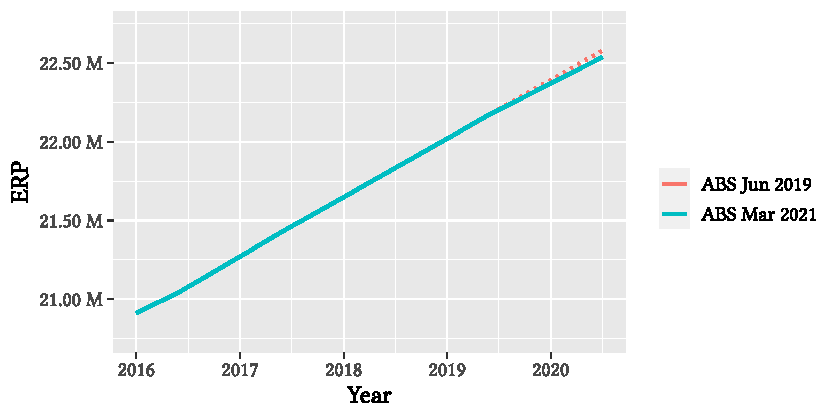
\includegraphics[height=0.75\textheight]{ref/pops-overall.pdf}
	\begin{flushright}\tiny\texttt{\url{https://www.abs.gov.au/statistics/people/population/national-state-and-territory-population}}\end{flushright}
\end{frame}

\begin{frame}{ABS Estimated Resident Population: Projected vs Reported 2}
	\center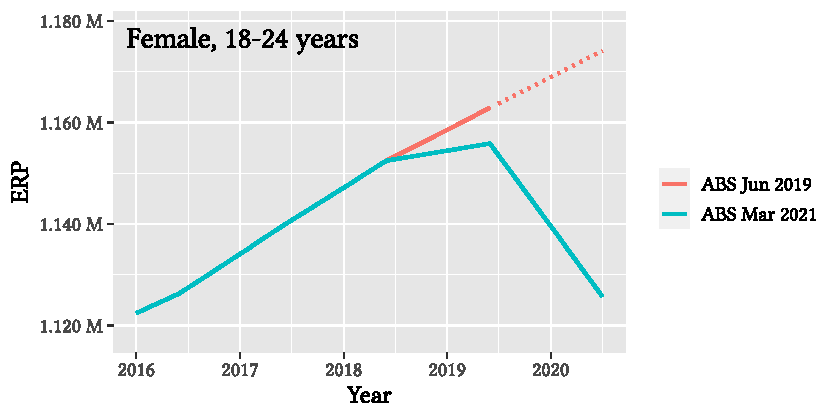
\includegraphics[height=0.75\textheight]{ref/pops-f18-24.pdf}
	\begin{flushright}\tiny\texttt{\url{https://www.abs.gov.au/statistics/people/population/national-state-and-territory-population}}\end{flushright}
\end{frame}

\begin{frame}{ABS components of population growth}

	\center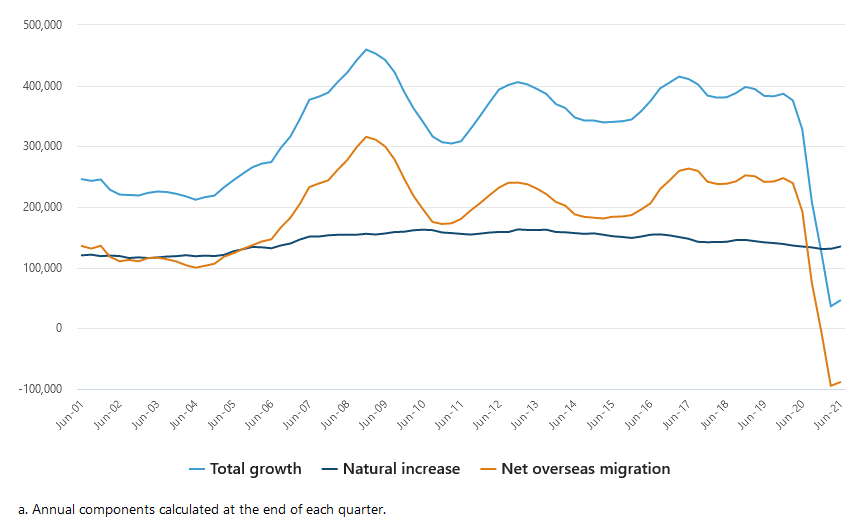
\includegraphics[height=0.75\textheight]{ref/pop-components.PNG}
	\begin{flushright}\tiny\texttt{\url{https://www.abs.gov.au/statistics/people/population/national-state-and-territory-population}}\end{flushright}
\end{frame}

\begin{frame}{Net overseas migration: PBS/MBS eligibility?}
	\center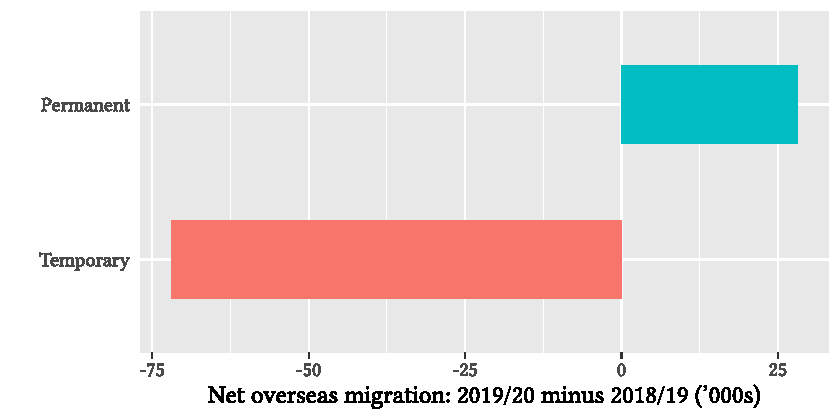
\includegraphics[height=0.75\textheight]{ref/pops-nom.pdf}
	\begin{flushright}\tiny\texttt{\url{https://www.abs.gov.au/statistics/people/population/migration-australia/latest-release}}\end{flushright}
\end{frame}


\begin{frame}{Finally}
	\begin{itemize}
		\item Remember they're \emph{estimated} resident populations
		\item As 2021 census results become available, 2017--2020 will be adjusted
	\end{itemize}
\end{frame}

\begin{frame}{Thanks}
    \begin{itemize}
        \item Juliana
        \item Andrea
    \end{itemize}
\end{frame}

\end{document}
